% (M5-M24) Leader: NCSR "D"
% CeADAR, UPC, ATOS, EVIDEN, FDI, INRIA, ARCADA, use case partners

\subsection{Introduction}

In this research, we aim to develop a task-agnostic framework for time-series data quality estimation. Towards this goal, we propose methods for anomaly and noise detection, which allow us to identify biased, noisy, inconsistent, or otherwise low-quality data, as well as data that may have been maliciously manipulated to contaminate the model during training.

As a case study to validate our methods, we use the Bitbrain dataset, which consists of EEG signals collected from a headband across 128 recordings. This headband includes two EEG channels synchronized with medical-grade EEG devices. The signals are annotated by three experts, with each 30-second segment classified into one of five sleep stages: Wake, N1, N2, N3, and REM. These stages correspond to specific brain activity patterns, such as slow eye movements, sleep spindles, and other characteristic waveforms.

To further validate the robustness of our proposed methods, we explore data augmentation techniques, including adversarial machine learning methods that introduce controlled noise contamination into the dataset.

\subsection{Problem Statement}

The quality of time-series data plays a crucial role in the performance of machine learning models, yet existing methods often fail to effectively identify and handle noise in a task-agnostic manner. Traditional data quality estimation techniques are typically tailored to specific datasets, limiting their applicability to a wider range of applications. 

In this research, we address this limitation by developing a flexible framework that estimates data quality, with respect to noise, anomalies, and malicious manipulation, across different time-series datasets, regardless of the specific task or domain. This approach is commonly referred to as task-agnostic data quality estimation.

\subsection{Proposed Methodology}

We propose a task-agnostic framework for time-series data quality estimation, using a combination of machine learning-based and statistical approaches to detect noise and anomalies in data. The primary techniques used in this framework include:

\begin{enumerate}
    \item[(a)] Unsupervised machine learning with autoencoders, which compress the data and detect noise based on reconstruction errors.\\
    \vspace{-0.8cm}
    \item[(b)] Supervised machine learning with a transformer model, which uses attention mechanisms to identify noisy segments in the data.\\
    \vspace{-0.8cm}
    \item[(c)] Statistical approaches which detect noise based on changes in data characteristics over time.
\end{enumerate}

To apply these techniques, we implement the following 8 methods: LSTM Autoencoder, Convolutional LSTM Autoencoder, Attention-based Autoencoder, Transformer, MNE Filtering, Cumulative Sum Control, Page-Hinkley Test and Kullback-Leibler Divergence. The last 3 statistical methods are implemented using the \href{https://github.com/IFCA-Advanced-Computing/frouros}{Frouros} framework.

In our analysis, we chose to estimate noise across 30-second segments of the EEG data, which, in the Bitbrain dataset, corresponds to 7,680 samples. Since each method outputs noise values in different scales, we transform these values into binary based on predefined thresholds per channel to establish a common ground for comparison.

\subsection{Machine Learning Approach}
The general concept of using machine learning (ML) for noise estimation revolves around training models to solve specific tasks and then using their outputs during inference to estimate noise. These tasks may vary in nature — ranging from signal reconstruction and prediction to classification — but the core idea is that the model’s performance on these tasks can be used to infer the presence of noise.

To train the models, we split the dataset into training (43 recordings), validation (3 recordings), and testing subsets (10 recordings). Noise estimation is performed using the test dataset. For the training configuration, we set the batch size to 512 and train the models for a maximum of 1000 epochs. To prevent overfitting, we employ early stopping with a patience of 30 epochs, meaning that if the validation loss does not improve for 30 consecutive epochs, training will stop. We set the learning rate to $1e^{-4}$ and use the Adam optimizer to adjust the model weights. Additionally, we implement a \emph{ReduceLROnPlateau} scheduler to dynamically adjust the learning rate based on the validation loss. If the validation loss plateaus, the scheduler reduces the learning rate to help the model continue improving.

To ensure robust model training and reliable outcomes, we rely on data preprocessing techniques. Proper preprocessing standardizes the input data, mitigates inconsistencies, and enhances the model’s ability to learn meaningful representations. In our case, preprocessing involves handling missing or ambiguous data by removing rows containing NaN values, as well as any samples where expert annotators could not agree on the class label (i.e., samples with a label value of 8). Additionally, we apply normalization to assist model training by making the data more uniform. Due to the low variability and the presence of extreme outliers in the EEG signals, we adopt a robust normalization approach. Instead of using the mean and standard deviation, which are sensitive to outliers, we use the median and interquartile range (IQR). We scale the data based on statistics computed across the entire dataset, rather than on a per-batch basis, since the statistics remain consistent across the full dataset.

\begin{equation}
    x_{\text{norm}} = \frac{x - \text{median}(x)}{\text{IQR}(x)} \label{eq:robust_norm}
\end{equation}

where $x$ represents the values of a particular feature, $\text{median}(x)$ is the median value of the feature, and $\text{IQR}(x)$ is the interquartile range, which measures the spread of the middle 50\% of the data. We use the median as a measure of central tendency because it is robust against extreme values, making it a more reliable indicator for our dataset, which exhibits low variability and where even small differences matter. Additionally, we use the interquartile range $\text{IQR} = Q_3 - Q_1$ to reduce the influence of outliers by focusing on the range within which the central portion of the data lies. This approach ensures that our normalization process allows the model to learn from the true patterns in the dataset.

For all machine learning methods, we need to establish a common standard to determine what is considered noise and what is not. As the models output different value ranges, we need a policy to classify these outputs into binary values that indicate noise presence or absence. One such approach involves defining thresholds that act as a boundary between noise and clean data. For these methods, we define thresholds based on the 75th percentile of noise values for each channel. Values above the thresholds are set to 1 (indicating noise), while those below are set to 0 (indicating no noise).

Noise estimation within this machine learning approach can be divided into two categories: label-based and label-free:

\begin{itemize}
    \item The label-based approach involves training classifier models on labeled data to learn how to assign class labels to signals. The \emph{Transformer Classifier}, trained to classify signals into sleep stages, belongs to this category. The idea is to use the model’s attention matrix, which highlights the importance of different time steps in data, to infer the presence of noise. Higher attention values correspond to segments of data that are likely noisy, whereas lower attention values indicate cleaner segments of data.
    \vspace{-0.2cm}
    \item The label-free approach does not rely on labeled data for training. Instead, it focuses on unsupervised or semi-supervised techniques to estimate noise based on the characteristics of the signal itself. In this category, we use models like autoencoders and transformers that learn to reconstruct or predict signals. The 3 \emph{Autoencoders} as well as the \emph{Transformer Predictor} are examples of models used in this approach. These models are trained to reconstruct the input data, and noise is mainly identified through the reconstruction error — the larger the error, the more likely the segment is noisy. Additionally, the attention-based models, \emph{Attention-based Autoencoder} and \emph{Transformer Predictor}, can also estimate noise using the attention matrix. Just like in the label-based approach, higher attention values indicate segments of data that are likely noisy, while lower attention values correspond to cleaner segments.
\end{itemize}

\subsubsection{LSTM Autoencoder}
....
Compresses the input signal into a latent representation and then attempts to reconstruct it. Noise is estimated as the difference between the original and reconstructed signals, hoping that only the non-noisy information is preserved during compression. 
....
We implement an LSTM-based autoencoder to transform the EEG signals into a lower-dimensional latent representation. The encoder consists of LSTM layers that capture the temporal patterns of the input sequence, while the decoder reconstructs the original signal from the latent representation. This architecture is chosen because LSTMs are well-suited for sequential data and can effectively model the temporal dependencies present in EEG signals.
....
We split each 30s segment into 32 chunks, so we end up with 7680/32=240 sequences in each chunk. The input, structured as sequences of length 240 with 2 features corresponding to the EEG channels, is processed by the encoder, which extracts temporal patterns and relationships within the data. This process results in a latent representation of size (1, 8), where the first dimension corresponds to a single compressed time step and the second dimension represents the 8 learned features.
...
To balance the models' focus on both the amplitude and trends of the EEG signals, we define a custom loss function, called \emph{BlendedLoss}. This function combines the median and mean of the powered absolute differences between the predicted ($\hat{x}$) and target values ($x$):
%
\begin{equation}
\text{Loss} = (1 - \text{blend}) \cdot \text{median}(\lvert \hat{x} - x \rvert^p) + \text{blend} \cdot \text{mean}(\lvert \hat{x} - x \rvert^p)
\label{eq:blended_loss}
\end{equation}
%
where $p$ is the power parameter that controls the sensitivity of the loss to the differences, $x$ is the original signal, and $\hat{x}$ is the reconstructed signal. The blend factor controls the trade-off between learning the overall trends (via the median) and capturing the amplitude (via the mean). We experiment with different blend values (0.1 and 0.8) to observe how this affects the model’s performance in reconstructing the signals.
....

\subsubsection{Convolutional LSTM Autoencoder}
...
The same \emph{BlendedLoss} function is used here as well, as defined in Equation~\ref{eq:blended_loss}.

\subsubsection{Attention-based Autoencoder}
...
The \emph{BlendedLoss} function as defined in Equation~\ref{eq:blended_loss}, is also used for the attention-based autoencoder, ensuring consistency across all autoencoders.

\subsubsection{Transformer}
....
%Classifies sleep stages using attention mechanisms. Noise is identified in parts of the signal that get lower attention scores during inference. These are less informative for feature-label associations, likely due to the disruptive effect of noise.
...
To train the model, we use Cross-Entropy loss, which measures the dissimilarity between the predicted probability distribution and the true distribution. This loss function is commonly used for classification problems to penalize the model based on how confident and accurate its predictions are. Given that the dataset is quite imbalanced, with class frequencies reflected by the weights as shown in Table \ref{tab:class_freqs_weights}, we employ a weighted version of the Cross-Entropy loss (see: Equation~\ref{eq:weighted_cross_entropy_loss}). This approach adjusts the influence of each class in the loss calculation, helping the model learn across all class distributions, regardless of their prevalence in the dataset.

\begin{equation}
    \text{Loss} = -\sum_{i=1}^{N} w_{y_i} \cdot \log(p_{y_i})
    \label{eq:weighted_cross_entropy_loss}
\end{equation}

where \(N\) is the total number of samples, \(y_i\) represents the true class label for the \(i\)-th sample, \(p_{y_i}\) is the predicted probability for the true class, and \(w_{y_i}\) is the weight assigned to the class \(y_i\).

\begin{table}[h!]
    \centering
    \begin{tabular}{c|c|c}
    Class & Freqs (\%) & Weights \\
    \hline
    0 & 14.11 & 0.12 \\
    1 & 4.45  & 0.39 \\
    2 & 62.16 & 0.03 \\
    3 & 4.96  & 0.35 \\
    4 & 14.36 & 0.12 \\
    \end{tabular}
    \caption{Class frequencies and weights used in weighted cross-entropy loss.}
    \label{tab:class_freqs_weights}
\end{table}

\subsection{Statistical Approach}
....
Preprocessing for the statistical methods is similar to that of the machine learning-based methods in terms of handling NaN values and ambiguous samples. However, unlike the machine learning methods, no normalization is applied, as the statistical methods require the raw data to function.
....
For MNE filtering, the noise thresholding approach is consistent with the machine learning-based methods, using the 75th percentile to separate noise (1) from no noise (0). On the other hand, the Frouros-based methods inherently provide binary outputs. To handle cases where sample aggregation results in float values, we apply a threshold of 0.5 to convert these results into binary form.
...
To ensure consistency across all methods and enable meaningful comparisons, the same test recordings used for machine learning-based noise estimation are also applied to the statistical methods.
... 

\subsubsection{MNE Filtering}
...
%Applies bandpass filtering to the input signals to remove noise outside a specified frequency range (0.5 to 40 Hz). Noise is estimated as the difference between the original and the filtered version.
....

\subsubsection{Cumulative Sum Control}
...

\subsubsection{Page-Hinkley Test}
...

\subsubsection{Kullback-Leibler Divergence}
...








\subsubsection{Cumulative Sum Control}
Tracks the cumulative sum of deviations from a target mean over time. Noise is detected when the cumulative sum of these deviations exceeds a threshold.

\subsubsection{Page-Hinkley Test}
Compares the cumulative mean of observed values to the global mean of the data. Noise is detected when the cumulative mean diverges from the global mean beyond a threshold.

\subsubsection{Kullback-Leibler Divergence}
Measures the difference between probability distributions of two consecutive data windows. Noise is estimated when the divergence exceeds a threshold.






%%%%%%%%%%%%%%%%%%%%%%%%%%%%%%%%%%%%%%%%%%%%%%%%%%%%%%%%%%%%%%%%%%%%%%%%%%%%%%%%%%%%%%%%%%%%%%%%%%%%%%%%%%%%%%%
% During the experiments, we focus on evaluating how well the decoder reconstructs the latent representations back into their original form. We compare the original signal with the decoded version, not only visually through plots but also by using various metrics to quantify performance. Since the testing data is quite large, we select one random batch for analysis. This batch is visualized using two subplots, one for each EEG feature, representing the signal for each channel separately.

% \subsection{Signal Comparison} First, we plot the original and decoded signals, where the x-axis represents the samples and the y-axis shows the amplitude of the signal.

% When the blend is set to 0.1, the decoded signal effectively captures the tendencies and patterns of the original signal, though its amplitude is significantly restricted, centering around zero. The original signal displays larger amplitudes, with values ranging from approximately 3 to -9.
% %
% \begin{figure}[ht]
%     \centering
%     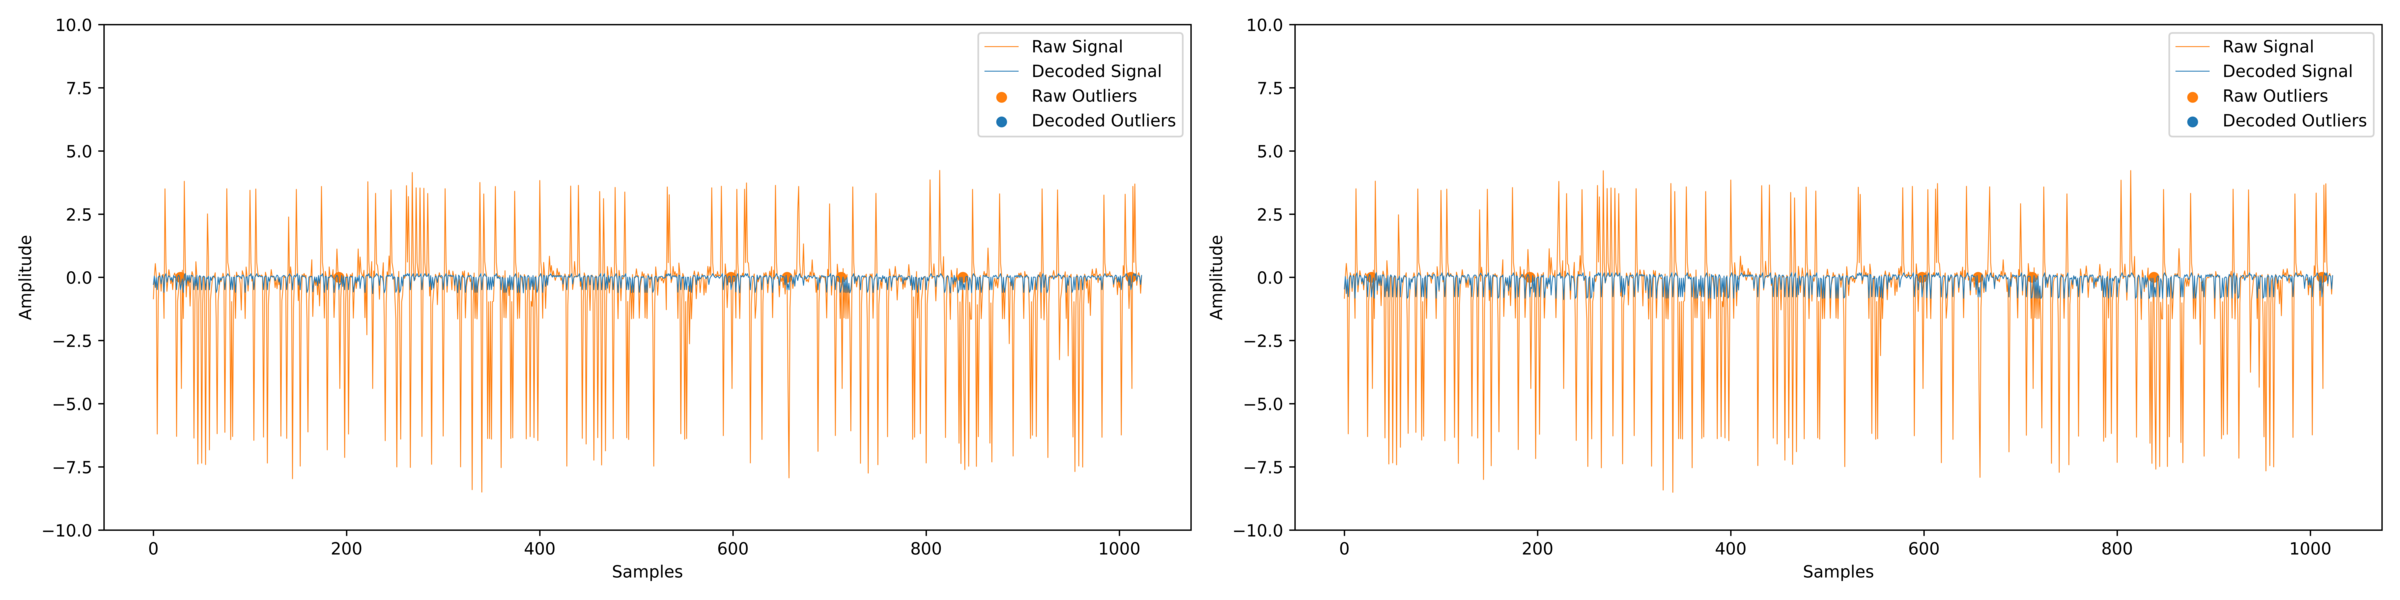
\includegraphics[width=0.8\textwidth]{static/original_vs_decoded_blend_01_resized.png}
%     \caption{Signals when blend=0.1}
%     \label{fig:signal_01}
% \end{figure}
% %
% When the blend is set to 0.8, the decoded signal captures the patterns and flow of the original signal more accurately, with amplitudes reaching up to approximately $\pm0.5$. This improvement demonstrates that increasing the focus on the mean in the loss function results in an overall better reconstruction of the original signal.
% %
% \begin{figure}[ht]
%     \centering
%     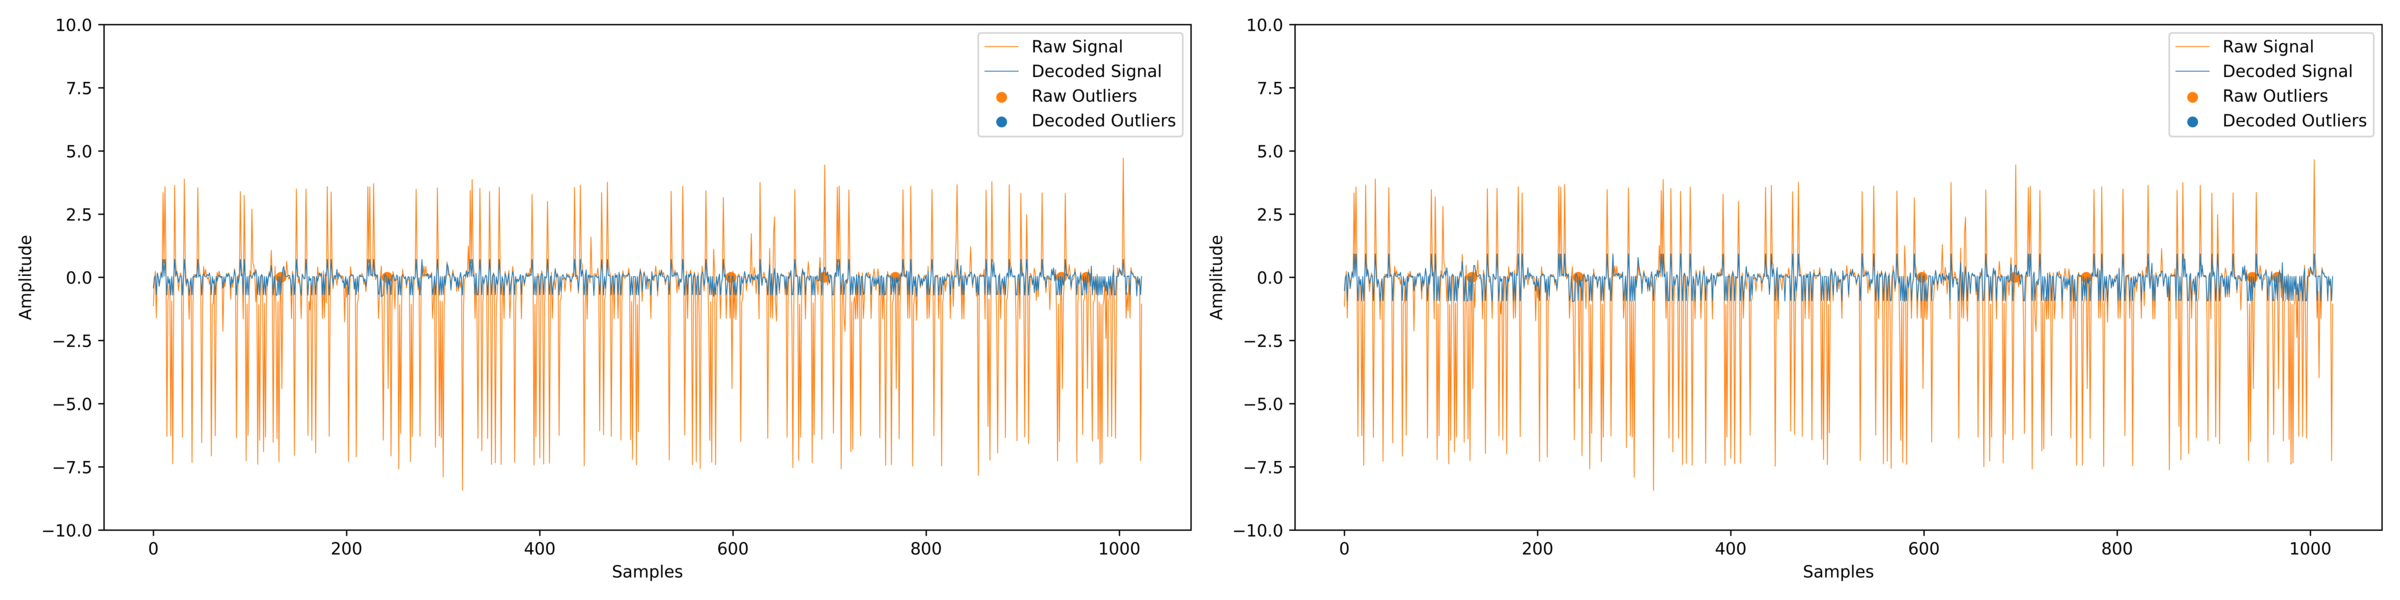
\includegraphics[width=0.8\textwidth]{static/original_vs_decoded_blend_08_resized.png}
%     \caption{Signals when blend=0.8}
%     \label{fig:signal_08}
% \end{figure}
% %

% \subsubsection{Detrended Signal Comparison} We also analyze the detrended signal using the Theil-Sen estimator. For both the 0.1 and 0.8 blends, the detrended signal trends are nearly flat, indicating minimal differences between the original and decoded signals.
% %
% \begin{figure}[ht]
%     \centering
%     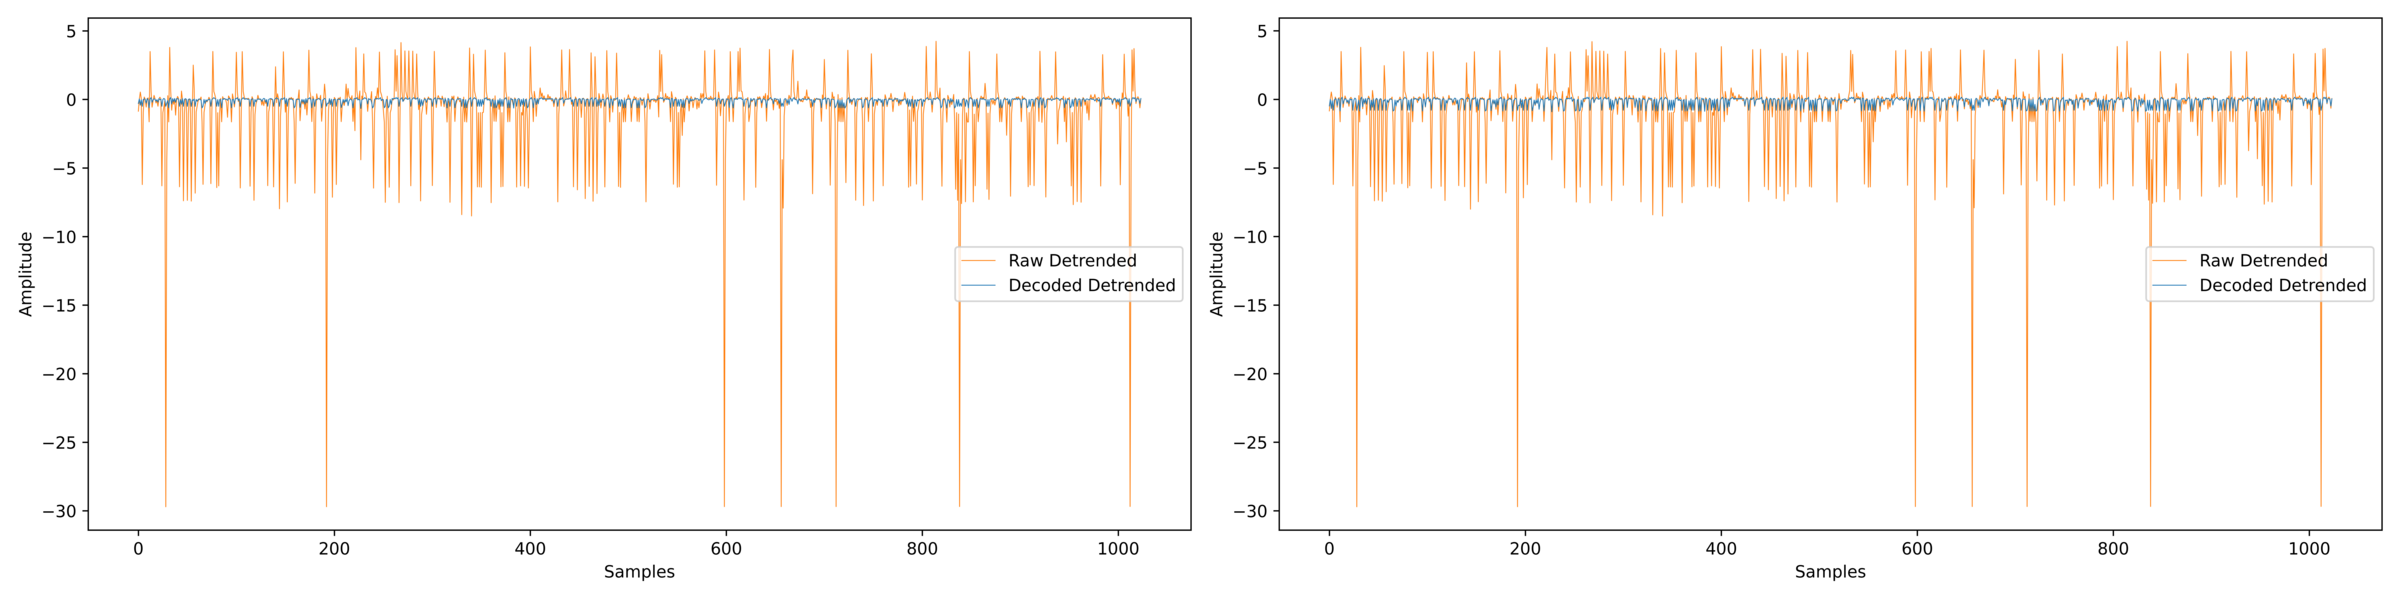
\includegraphics[width=0.8\textwidth]{static/detrended_signal_blend_01_resized.png}
%     \caption{Detrended signals when blend=0.1}
%     \label{fig:detrended_signal_01}
% \end{figure}
% %

% %
% \begin{figure}[ht]
%     \centering
%     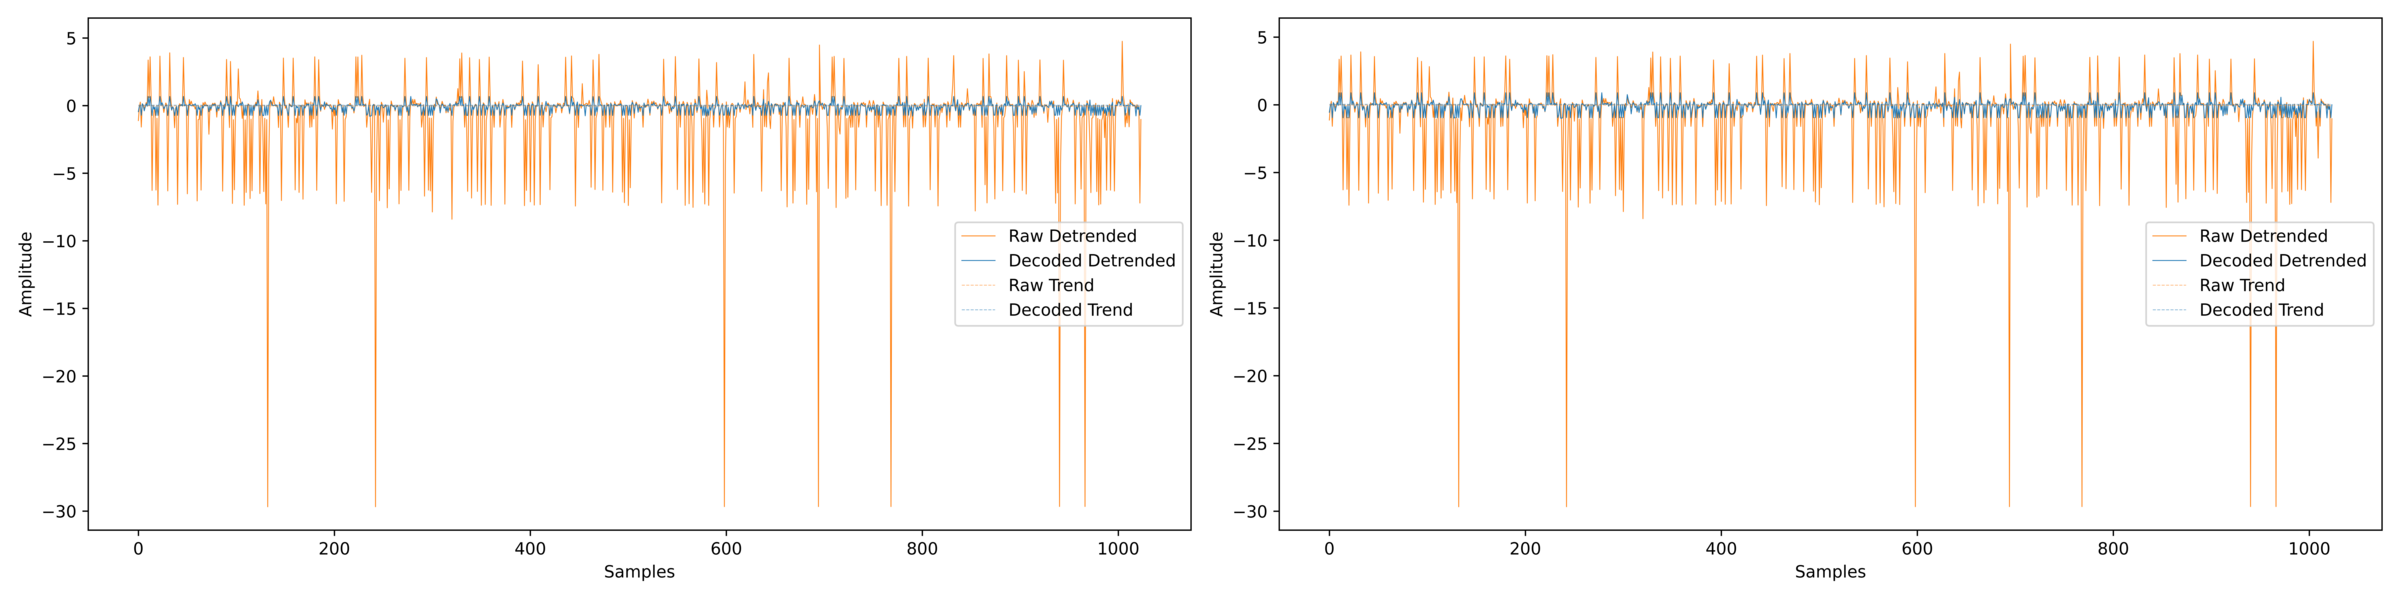
\includegraphics[width=0.8\textwidth]{static/detrended_signal_blend_08_resized.png}
%     \caption{Detrended signals when blend=0.8}
%     \label{fig:detrended_signal_08}
% \end{figure}
% %

% \subsubsection{RMS Analysis} The root mean square (RMS) analysis provides additional insight into the performance of the autoencoder. When the blend is set to 0.1, the majority of the RMS values are centered around zero, with outliers remaining prominent. This result is acceptable but suggests room for improvement. When the blend is set to 0.8, the RMS shows significant improvement, with a higher count of zeros. The outliers continue to exhibit significant values, but overall, the analysis indicates a better reconstruction.
% %
% \begin{figure}[ht]
%     \centering
%     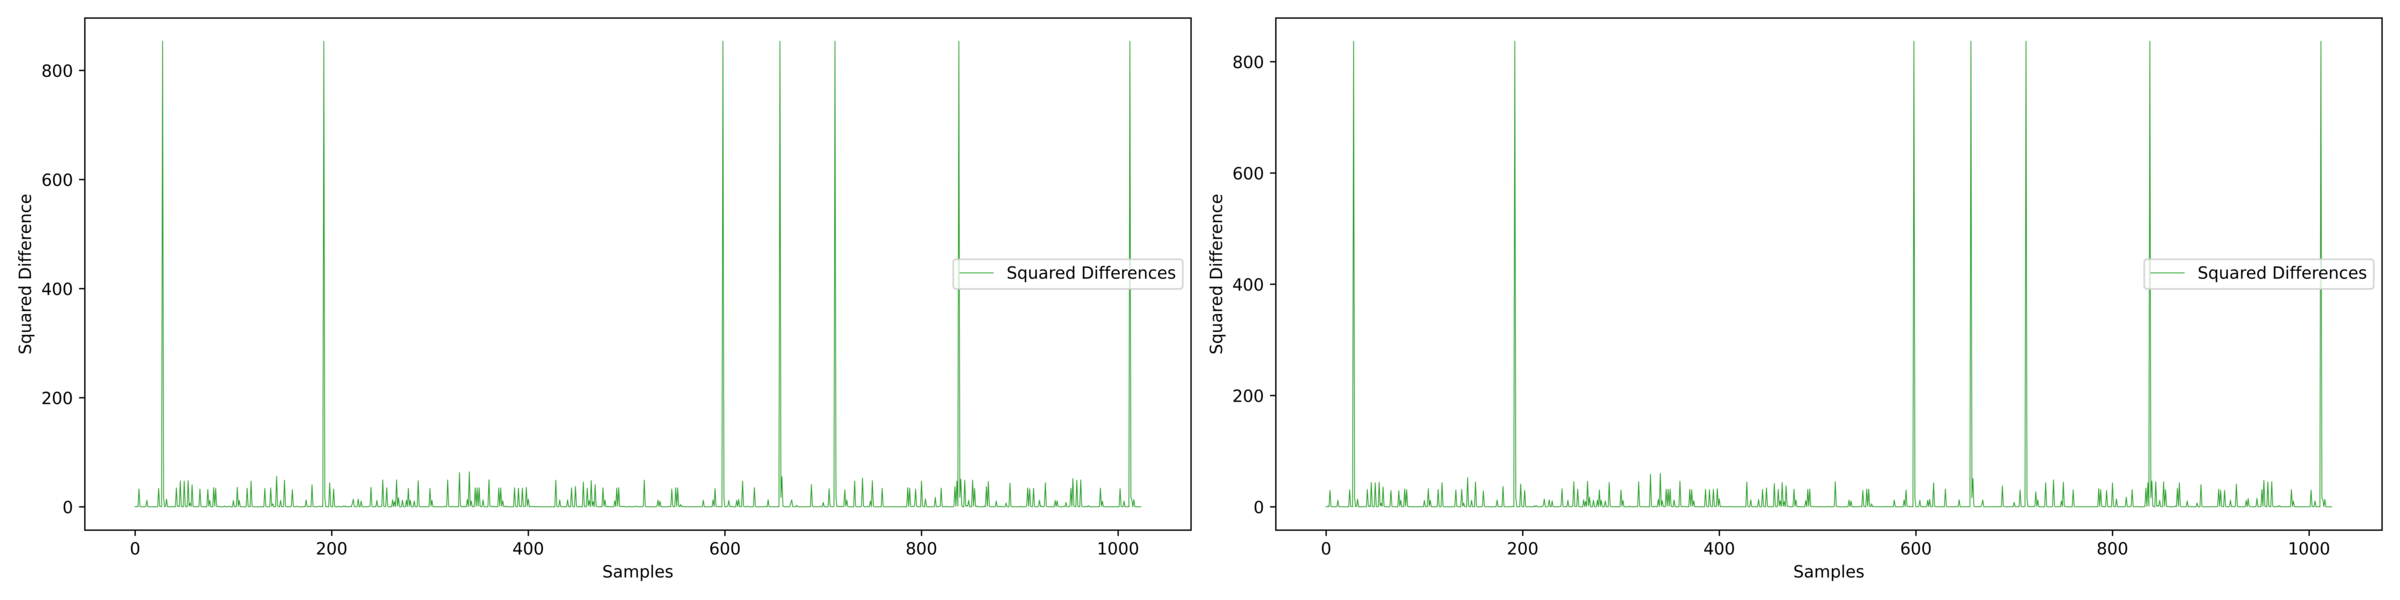
\includegraphics[width=0.8\textwidth]{static/rms_analysis_blend_01_resized.png}
%     \caption{RMS analysis when blend=0.1}
%     \label{fig:rms_analysis_01}
% \end{figure}
% %

% %
% \begin{figure}[ht]
%     \centering
%     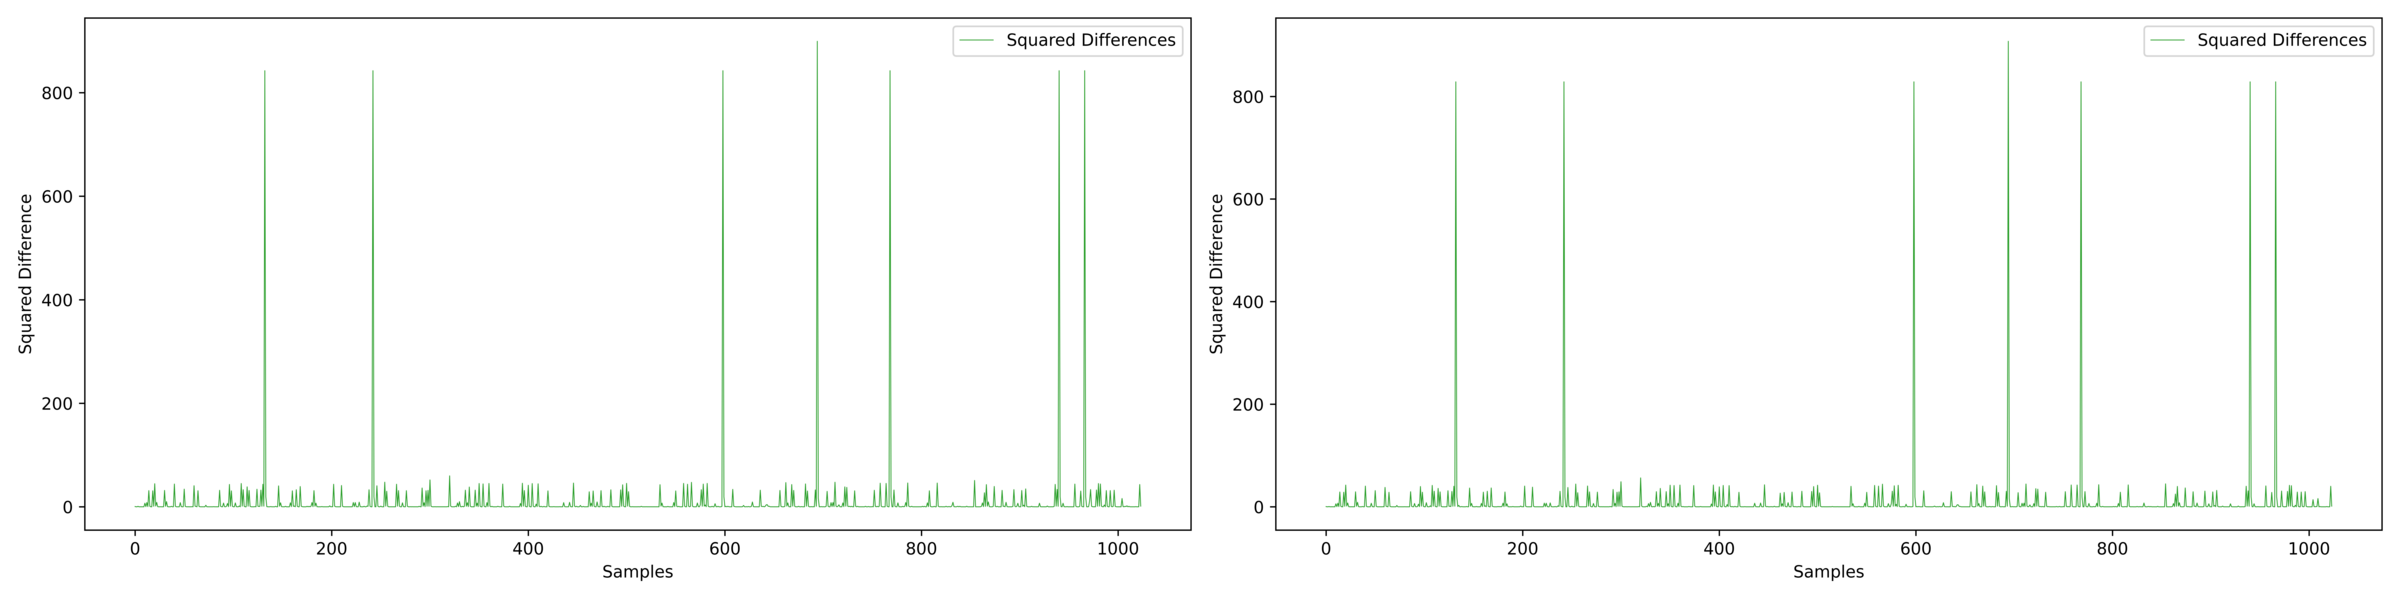
\includegraphics[width=0.8\textwidth]{static/rms_analysis_blend_08_resized.png}
%     \caption{RMS analysis when blend=0.8}
%     \label{fig:rms_analysis_08}
% \end{figure}
% %

% \subsubsection{Band Analysis} When the blend is set to 0.8, the decoded signal exhibits non-zero values across all bands, indicating a more robust amplitude representation. In some bands, the levels of the decoded signal closely match those of the original signal, suggesting that the model effectively captures the corresponding frequency ranges. In contrast, when the blend is set to 0.1, the distributions of the raw and decoded bands differ significantly. Some bands in the decoded signal are nearly zero, while the raw signal contains substantial values, indicating that the amplitude is not well captured.
% %
% \begin{figure}[ht]
%     \centering
%     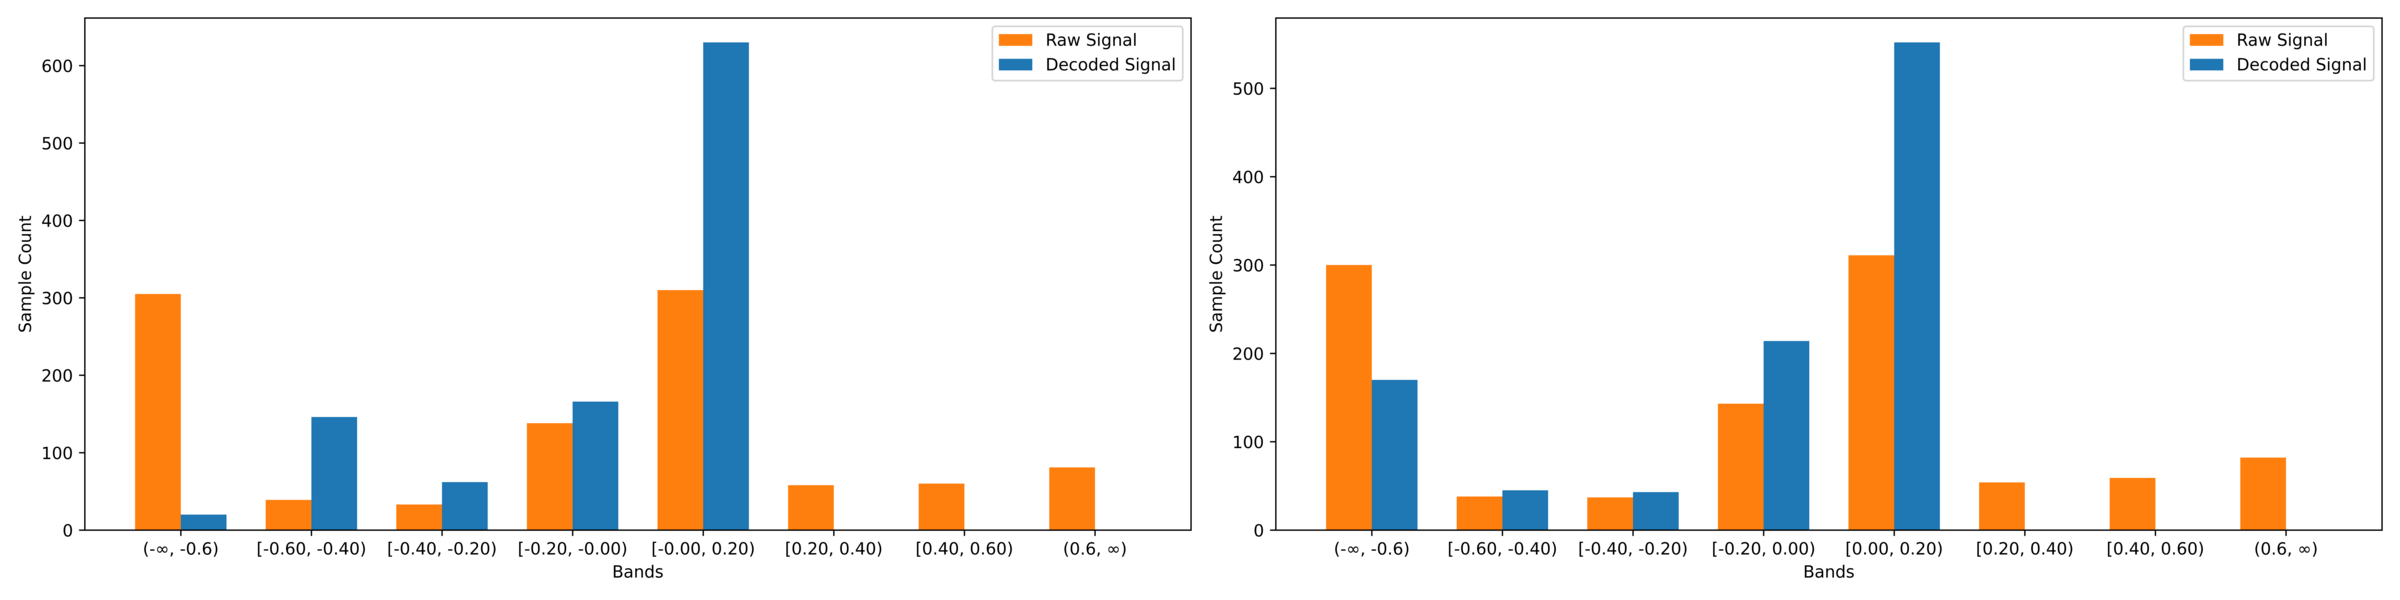
\includegraphics[width=0.8\textwidth]{static/band_analysis_blend_01_resized.png}
%     \caption{Band analysis when blend=0.1}
%     \label{fig:band_analysis_01}
% \end{figure}
% %

% %
% \begin{figure}[ht]
%     \centering
%     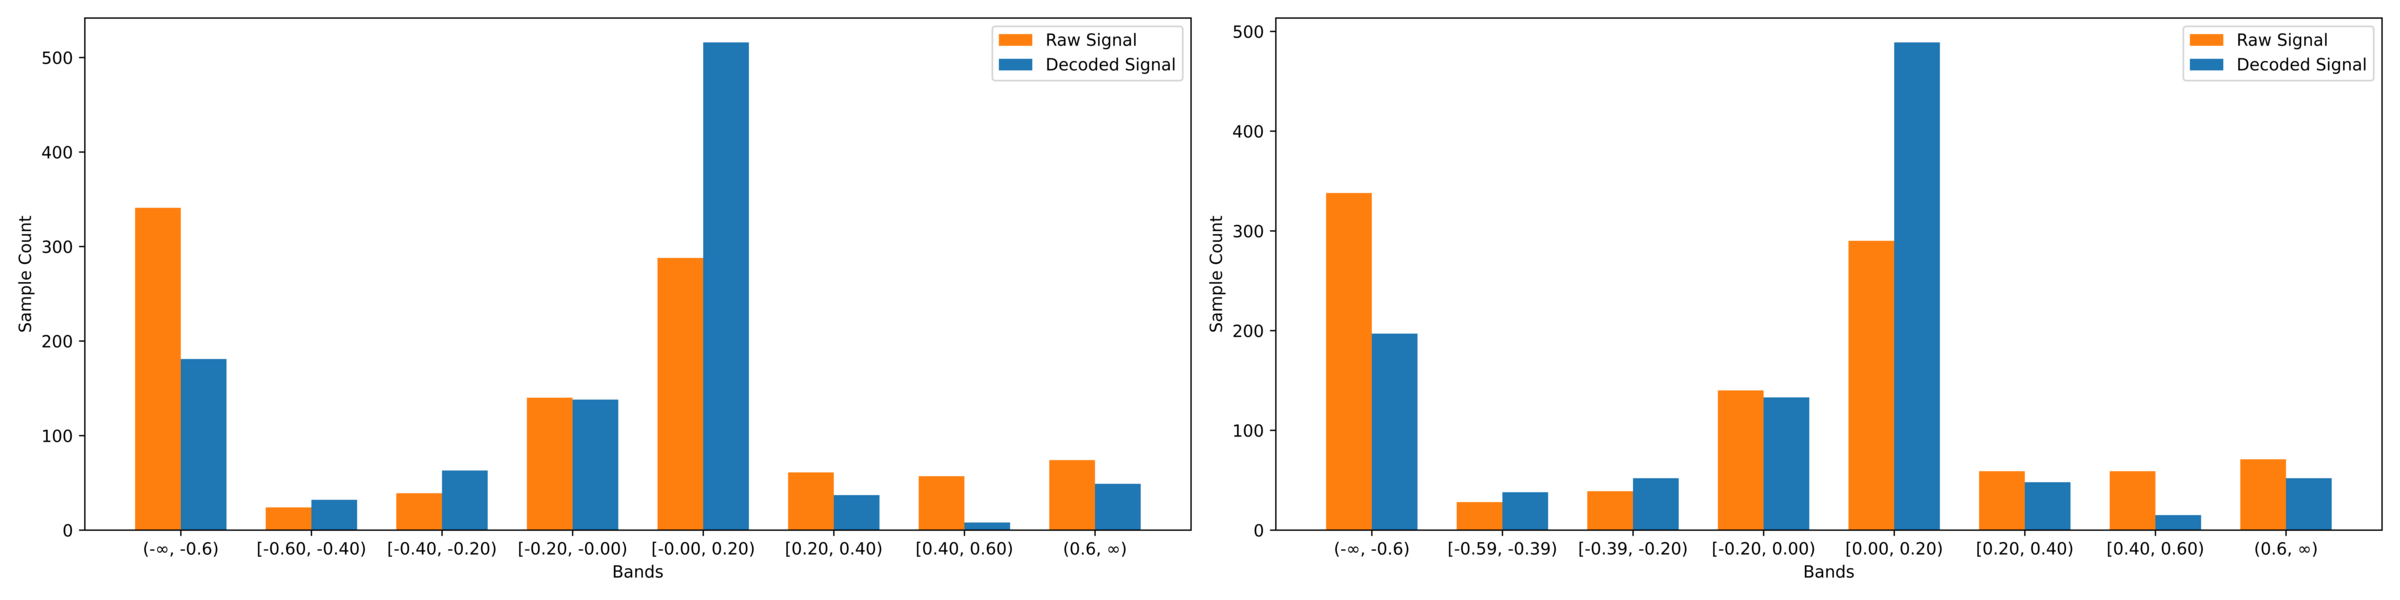
\includegraphics[width=0.8\textwidth]{static/band_analysis_blend_08_resized.png}
%     \caption{Band analysis when blend=0.8}
%     \label{fig:band_analysis_08}
% \end{figure}
% %

% \subsubsection{Other Metrics}

% The performance of the autoencoder is evaluated using various metrics for both blends (0.1 and 0.8). These metrics include band rate differences, zero-crossing rates, RMS values, and Pearson correlation coefficients, calculated as differences between the raw and decoded signals. A smaller difference indicates a closer match to the original signal, which is preferable. Better results are highlighted in blue. Below are the detailed results for each feature and blend setting, showing that the blend with 0.8 is superior.
% %
% \begin{table}[ht]
%     \centering
%     \begin{tabular}{l|c|c}
%         \hline
%         \textbf{Metric} & \textbf{Blend=0.8} & \textbf{Blend=0.1} \\ 
%         \hline
%         Bands \% $F_1$ & 
%         \begin{tabular}[c]{@{}c@{}} 
%         \color{blue}{0.4422} \\ 
%         1.0 \\ 
%         1.0 \\ 
%         -0.1232 \\ 
%         \color{blue}{0.3420} \\ 
%         1.0 \\ 
%         1.0 \\ 
%         \color{blue}{0.3108} 
%         \end{tabular} 
%         & 
%         \begin{tabular}[c]{@{}c@{}} 
%         0.9557 \\ 
%         1.0 \\ 
%         1.0 \\ 
%         \color{blue}{-0.2767} \\ 
%         0.7927 \\ 
%         1.0 \\ 
%         1.0 \\ 
%         1.0 
%         \end{tabular} \\
%         \hline
        
%         Bands \% $F_2$ & 
%         \begin{tabular}[c]{@{}c@{}} 
%         \color{blue}{0.3659} \\ 
%         1.0 \\ 
%         1.0 \\ 
%         \color{blue}{-0.0824} \\ 
%         \color{blue}{0.2217} \\ 
%         1.0 \\ 
%         1.0 \\ 
%         \color{blue}{0.2556} 
%         \end{tabular} 
%         & 
%         \begin{tabular}[c]{@{}c@{}} 
%         0.4524 \\ 
%         1.0 \\ 
%         1.0 \\ 
%         -0.2741 \\ 
%         0.7840 \\ 
%         1.0 \\ 
%         1.0 \\ 
%         1.0 
%         \end{tabular} \\
%         \hline

%         Zero Crossing Rate $F_1$ & 1.3439 & \color{blue}{1.2631} \\ 
 
%         Zero Crossing Rate $F_2$ & 1.3334 & \color{blue}{1.0186} \\ 
 
%         RMS $F_1$ & \color{blue}{2.8682} & 2.9533 \\ 

%         RMS $F_2$ & \color{blue}{2.7980} & 2.8774 \\ 
  
%         Pearson Correlation $F_1$ & \color{blue}{0.6527} & 0.6085 \\ 
   
%         Pearson Correlation $F_2$ & \color{blue}{0.6610} & 0.6364 \\ 
%         \hline
%     \end{tabular}
%     \caption{Comparison of Metrics for Blends 0.1 and 0.8. Metrics are expressed as differences between Raw and Decoded signals.}
%     \label{tab:metrics_comparison}
% \end{table}
% %